\chapter{Coherencia entre la métrica transcripcional y otros espacios de conocimiento (GO)}
Esperamos que los conocimientos (entendidos como nociones de similitud) de los distintos espacios (el de expresión y el biológico) sean diferentes pero no ortogonales. Por lo tanto, una vez detectadas las estructuras en distintas resoluciones en el espacio de expresión, nos interesará cuantificar la congruencia biológica de las mismas. Para ello haremos uso de varios índices, BHI, BHI IC, BHIl índice de homogeneidad biológica (o BHI por sus siglas en inglés) de una partición, introducido por Datta \cite{Datta2006}. Este observable cuantifica el grado en que una partición presenta grupos biológicamente homogéneos, reportando, para cada grupo, la máxima proporción de pares de genes agrupados que comparten una misma clase funcional de Ontología Génica. Consideremos dos genes $x$ e $y$ que pertenecen a un mismo grupo $D$ de una partición dada, con un total de $k$ grupos, y sean $C(x)$ y $C(y)$ los conjuntos de todas las clases funcionales que tienen anotados a los genes $x$ e $y$ respectivamente. Sea además la función indicadora $I(C(x)=C(y))$ que toma el valor $1$ si hay al menos una clase en donde ambos genes estén anotados, y $0$ en caso contrario. Entonces, el índice de homogeneidad biológica queda definido como:
\begin{equation}
	BHI = \frac{1}{k}\sum\limits_{j=1}^k\frac{1}{n_j(n_j-1)}\sum\limits_{x\neq y\in D_j}I(C(x)=C(y))
\end{equation}
con $n_j$ la cantidad de genes anotados en el grupo $D_j$.\\
Los valores de BHI calculados para cada uno de los grupos del tratamiento ``frío'' en las particiones k-means (puntos rojos), $deepsplit=1$ (triángulos verdes) y $deepsplit=4$ (cuadrados azules) se presentan en la figura \ref{fig:bhi_km_ds1_ds4} junto con un control nulo consistente en 1000 reasignaciones aleatorias de las etiquetas de cada partición. Los grupos fueron ordenados según su masa de forma creciente.\\
Se observa que de los dos grupos de kmeans, solo uno presenta un BHI superior al tercer cuartil para el control nulo, mientras que para $deepsplit=1$, solo el 30\% de los grupos lo superan.
\begin{figure}[h]
    \centering
    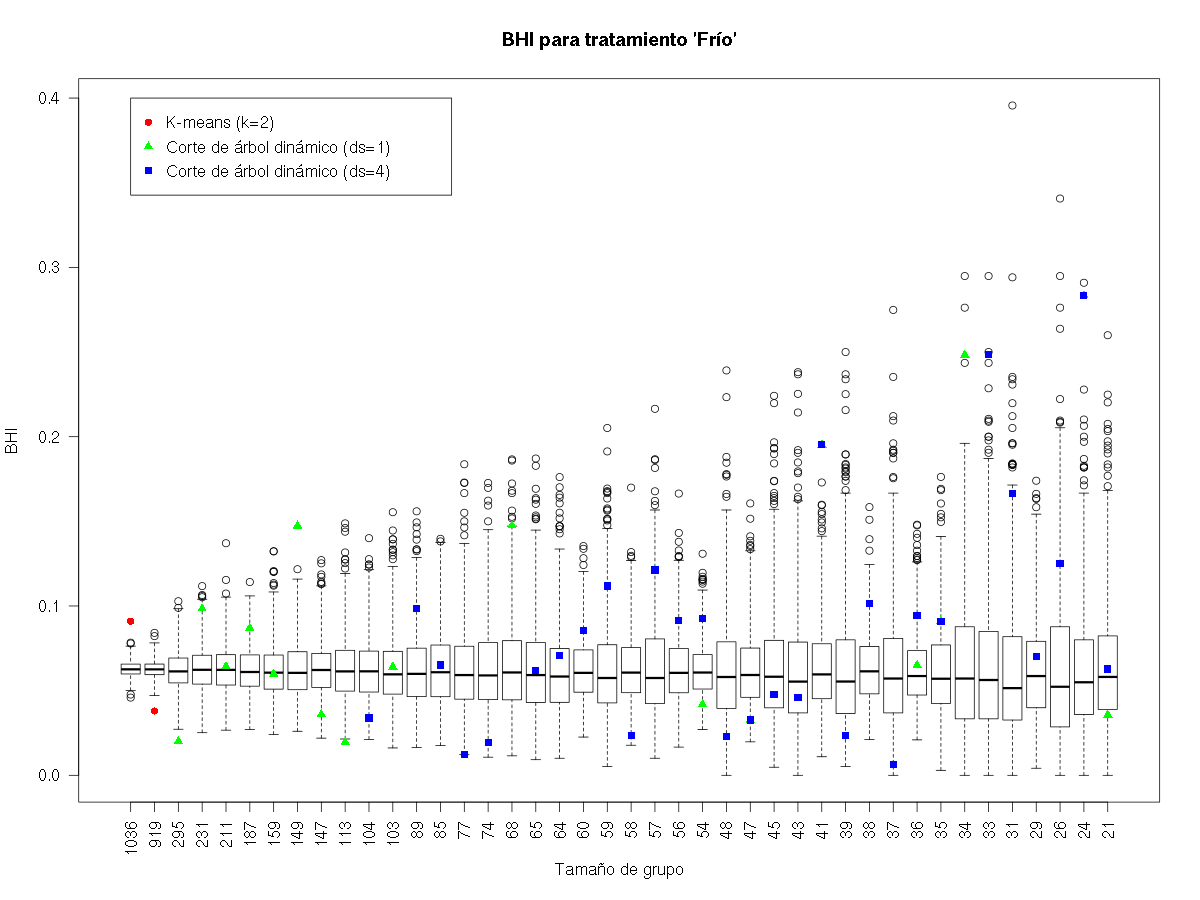
\includegraphics[width=0.8\textwidth]{bhi_km_ds1_ds4}
    \caption{Índice de Homogeneidad Biológica, BHI, para cada uno de los grupos del tratamiento 'Frío' obtenidos con kmeans, $deepsplit=1$ y $deepsplit=4$.}
    \label{fig:bhi_km_ds1_ds4}
\end{figure}
Finalmente, para la partición $deepsplit=4$, el BHI del 40\% de los grupos se encuentra por sobre el tercer cuartil del control nulo. Esto sugiere que si bien el aumentar la granularidad de la partición con el método corte de árbol dinámico resulta en un aumento de la consistencia biológica global de las estructuras observadas, esto no implica que las resoluciones utilizadas sean las óptimas.
\section{Discusión}
\hl{Ojo que esto quedo de la discusion del capitulo anterior}
En el presente análisis de estructura de los grupos obtenidos por medio de los métodos k-means, $deepsplit=1$ y $deepsplit=4$, encontramos que todos los métodos producen particiones altamente coherentes, con el método k-means generando las particiones más gruesas y los métodos subsiguientes, refinamientos de las mismas. La alta coherencia detectada es indicativo de que cada método logra  hallar estructuras en el espacio de expresión génica, aunque no siempre es factible realizar una interpretación biológica de las estructuras encontradas. Sobre todo en los grupos encontrados con k-means, que solamente toman en cuenta la expresión o inhibición de los genes. Sin embargo, el análisis de BHI indica que el aumentar la resolución con corte de árbol dinámico tampoco consigue encontrar la escala óptima en el análisis.\\
En el capitulo siguiente introduciremos algunas herramientas que buscarán cuantificar la homogeneidad biológica de particiones para encontrar dicha escala.